\subsection{eBPF Subsystem}
\label{subsec:ebpf_subsystem}
\textit{Note: The following subsection on background for eBPF is by and large taken from a previous project I made.\cite{ebpf-fuzz}}
\subsubsection{eBPF Programming Model}
% Will cover learning objective ``Explain the eBPF subsystem, in particular the machine- and programming model''.

Extended Berkeley Packet Filters (eBPF) is a subsystem in the Linux kernel. Originally introduced as Berkeley Packet Filters, now Classic Berkeley Packet Filters (cBPF)\cite{cBPF-paper}, the purpose was to allow effective filtering of network packets by enabling user space loading of packet filters that would execute in kernelspace. eBPF massively extends this idea and allows for many different types of programs to be loaded from user space and executed in kernel space.


The eBPF subsystem roughly consists of 5 different parts: eBPF programs, eBPF maps, the eBPF verifier which also does patching/rewriting of instructions, an interpreter and a collection of JIT compilers.



A rough overview of the interconnectedness of the eBPF subsystem can be seen in figure \ref{fig:ebpf-overview}. All userspace interactions with the eBPF subsystem, e.g. CRUD-operations on maps, loading and attaching of programs happen through the \verb!bpf! syscall. 
eBPF employs an event driven programming model: A user space process can load eBPF bytecode, which will trigger the verifier. On successful verification a file descriptor for the eBPF program is returned to the user space process, which in turn can be used to attach the program to a eBPF hook point. A hook point can be e.g. a system call or, in the case of packet filters, a socket. Once the program is verified, loaded and attached to a hook point, it will execute whenever the hook is triggered.
There are many eBPF program types, e.g. \verb!BPF_PROG_TYPE_SOCKET_FILTER! for filtering network packets, \verb!BPF_PROG_TYPE_KPROBE! for filtering kernel probes and \verb!BPF_PROG_TYPE_PERF_EVENT! for filtering calls to perf event handlers. The respective program types all have their own set of available hook points, i.e. a \verb!BPF_PROG_TYPE_SOCKET_FILTER! can be attached to a socket and triggered on incoming packets, a \verb!BPF_PROG_TYPE_PERF_EVENT! can be attached to perf events and triggered before the perf event handler is called etc.

For this project about proof carrying code, the program type is not relevant. The experiments in section \ref{sec:experiments} use the program type \verb!BPF_PROG_TYPE_SOCKET_FILTER! but this is mainly due to the convenience of being able to load socket filters as a non-root user. 
% In the case of this project, the eBPF programs will be of the socket filter type and the hook point will be a socket, such that the program is triggered to execute whenever a packet is received on the attached socket. 

\begin{figure}[htbp!]
  \centering
  \begin{tikzpicture}
    \node at (0,9) {User Space};
    \node at (0,7) {Kernel Space};
    % Line that splits user and kernel space
    \draw (0,8) -- (2,8);    
    \draw (5,8) -- (6,8);
    \draw (10,8) -- (11.5,8);    
    \draw (14.5,8) -- (16,8);
    % eBPF maps box
    \draw (11,4) -- (11,6) -- (15,6) -- (15,4) -- cycle;
    \node at (13,5) {eBPF maps};
    % eBPF bytecode box
    \draw (1.5,10.5) -- (5.5,10.5) -- (5.5,11.5) -- (1.5,11.5) -- cycle;
    \node at (3.5,11) {eBPF bytecode};
    % Process box
    \draw (6,13) -- (10,13) -- (10,14) -- (6,14) -- cycle;
    \node at (8,13.5) {Process};
    % Arrows
    \draw [stealth-stealth](6,13.5) -- (3.5,13.5) -- (3.5,11.5);
    \draw [stealth-stealth](10,13.5) -- (13,13.5) -- (13,8.5);
    \draw [stealth-stealth](13,7.5) -- (13,6);
    \draw [stealth-stealth](3.5,8.5) -- (3.5,10.5);
    \draw [stealth-stealth](3.5,7.5) -- (3.5,6);
    \draw [-stealth](8,13) -- (8,8.5);
    % Attach program box
    \draw (6,7.5) -- (6,8.5) -- (10,8.5) -- (10,7.5) -- cycle;
    \node at (8,8) {Attach Program};
    % Map helpers box
    \draw (11.5,7.5) -- (11.5,8.5) -- (14.5,8.5) -- (14.5,7.5) -- cycle;
    \node at (13,8) {Map helpers};
    % Load program box
    \draw (2,7.5) -- (2,8.5) -- (5,8.5) -- (5,7.5) -- cycle;
    \node at (3.5,8) {Load Program};
    % eBPF Verifier box
    \draw (1.5,6) -- (5.5,6) -- (5.5,4) -- (1.5,4) -- cycle;
    \node at (3.5,5) {eBPF verifier};
    % eBPF program box
    \draw (6.5,6) -- (10,6) -- (10,4) -- (6.5,4) -- cycle;
    \node at (8.3,5.5) {eBPF Program};
    \node at (8.3,4.5) {(Loaded)};    
    \draw [-stealth](5.5,5) -- (6.5,5);                    
    \draw [stealth-stealth](10,5) -- (11,5);
    % Socket box
    \draw (6.5,3) -- (10,3) -- (10,1) -- (6.5,1) -- cycle;
    \node at (8.3,2.5) {Socket};
    \node at (8.3,1.5) {(Hook Point)};
    \draw [-stealth] (8,3) -- (8,4);
    % \draw [-stealth] (8.5,3) -- (8.5,4);
    \draw [-stealth] (8,7.5) -- (8,6);        
  \end{tikzpicture}
  \caption{Rough overview of eBPF subsystem}
  \label{fig:ebpf-overview}
\end{figure}



% \subsubsection{eBPF Machine Model}
\subsubsection{eBPF ISA}

% \subsubsection*{eBPF instruction set}


The eBPF instruction set architecture includes 10 64-bit wide read/write registers \verb!R0! through \verb!R9!, 1 64-bit wide read-only register \verb!R10! containing a frame pointer and an instruction set that can be thought of as a stripped down version of \verb!x86_64!. 

The complete instruction set can be found at \cite{kernel:ebpf-inst} and an unofficial reference for valid eBPF opcodes is available at \cite{ebpf-unoff-spec}.
Almoste all eBPF instructions are 8 bytes and encoded as seen in Figure \ref{fig:ebpf-encoding}. In the case of loading 64-bit immediate values, the instruction is encoded as two 8 byte blocks and the 16 bytes are interpreted as a single instruction.


\begin{figure}[htbp!]
  \centering
  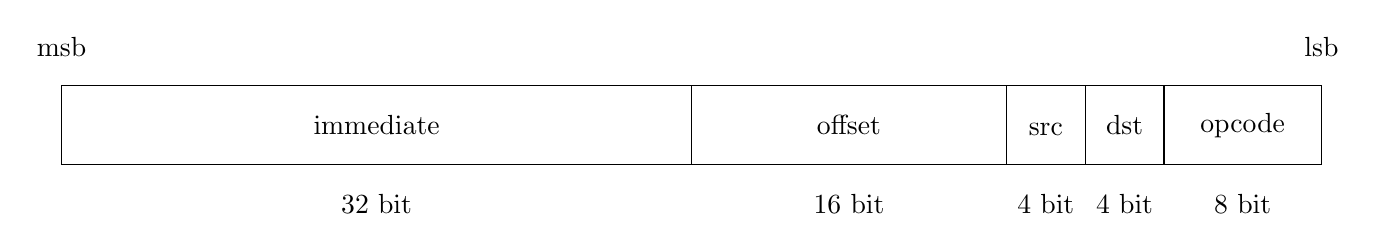
\begin{tikzpicture}
    \draw (0,0) -- (16,0) -- (16,1) -- (0,1) -- cycle;
    \draw (8,0) -- (8,1);
    \draw (12,0) -- (12,1);
    \draw (13,0) -- (13,1);
    \draw (14,0) -- (14,1);
    \node at (0,1.5) {msb};
    \node at (16,1.5) {lsb};
    \node at (4,0.5) {immediate};
    \node at (4,-0.5) {32 bit};    
    \node at (10,0.5) {offset};
    \node at (10,-0.5) {16 bit};    
    \node at (12.5,0.45) {src};
    \node at (12.5,-0.5) {4 bit};
    \node at (13.5,0.5) {dst};
    \node at (13.5,-0.5) {4 bit};    
    \node at (15,0.5) {opcode};
    \node at (15,-0.5) {8 bit};    
  \end{tikzpicture}
  \caption{The encoding of an eBPF instruction}
  \label{fig:ebpf-encoding}
\end{figure}




\subsubsection*{eBPF Maps}

eBPF maps are data structures accessible from both kernel space and user space.
There are several different types of maps available, e.g. stacks, queues, hash-tables and arrays.
All types of maps have four attributes\footnote{All attributes are not necessarily used or meaningful for all map types but required nonetheless. E.g. the stack map type has no use for a key, thus no use for a key size.}, as seen in Figure \ref{snip:map_struct}: The type of map, the maximum number of elements in the map, the size in bytes of keys used for indexing and the size in bytes of each value in the map. On successful creation of a map, a file descriptor is returned, which can then be used to refer to the map. 

\begin{figure}[htbp!]
  \centering
  \inputminted[linenos]{C}{snippets/map_struct.c}
  \caption{The struct used for creating a map, from \texttt{man(2) bpf}.}
  \label{snip:map_struct}
\end{figure}

% \textbf{TODO: The below on general ops is not true, e.g. for stack maps. Update text to make it correct}. \\

Maps support 5 general operations\footnote{According to \texttt{man bpf(2)}}, although not all map types support all the operations:
\begin{itemize}
\item \verb!BPF_MAP_CREATE!
\item \verb!BPF_MAP_LOOKUP_ELEM!
\item \verb!BPF_MAP_UPDATE_ELEM!
\item \verb!BPF_MAP_DELETE_ELEM!
\item \verb!BPF_MAP_GET_NEXT_KEY!  
\end{itemize}

In this project I have only used the eBPF map type \verb!BPF_MAP_TYPE_ARRAY! and in the following I will focus solely on that map type and related kernel helper functions.
The array map is a contiguous block of bytes, pre-allocated and zero-initialised, similar to arrays in e.g. \verb!C!. It supports the \verb!BPF_MAP_CREATE!, \verb!BPF_MAP_LOOKUP_ELEM! and \verb!BPF_MAP_UPDATE_ELEM! operations.

In user space lookups require the user to supply a buffer of the same size as the values in the map. On a successful lookup, the corresponding value will then be copied to the supplied buffer, such that the value is accessible in user space. An example of performing a lookup in a map can be seen in figure \ref{snip:map_lookup}. Similarly for updates, the new value must be supplied in a buffer, as can be seen in figure \ref{snip:map_update}. 


\begin{figure}[htbp!]
  \centering
  \inputminted[linenos]{C}{snippets/map_lookup_struct.c}
  \caption{Example of performing lookups in a map from user space applications, from \texttt{man(2) bpf}.}
  \label{snip:map_lookup}
\end{figure}

\begin{figure}[htbp!]
  \centering
  \inputminted[linenos]{C}{snippets/map_update_struct.c}
  \caption{Example of performing updates in a map from user space applications, from \texttt{man(2) bpf}.}
  \label{snip:map_update}
\end{figure}

In kernel space however, a successful lookup returns a pointer to the beginning of the value indexed by the supplied key. As long as this pointer points to memory that is part of the \textit{value} referenced by the \textit{key} used to obtain the original pointer, the pointer is valid in eBPF and can be used to read and write memory. As an example, if the value size of elements in a map are 16 bytes, to read the whole value the eBPF program must first obtain a pointer to the value, read the first 8 bytes, then increment the pointer by 8 and read the remaining 8 bytes of the value.


\subsubsection{eBPF Verifier - actions and guarantees}
% Will cover learning objective ``Explain the functionality of the eBPF verifier and what it guarantees''.
% Will cover learning objective ``Analyze and identify problems related to untrusted code (and sandboxing?)''

% \subsubsection*{eBPF Verifier and rules for eBPF programs}

The purpose of the eBPF verifier is to determine the safety of a eBPF program and whether it should be allowed to run.
Safe eBPF programs must follow a set of rules which are only informally defined and documented in a scattered manner. Documentation is available at the verifier subpage for the Linux kernel documentation\cite{ebpf-verifier}, in a text file located in the Linux kernel's networking documentation\cite{ebpf-filter} and as comments in the source code for the verifier itself
\texttt{/kernel/bpf/verifier.c}\cite{ebpf-verifier-source}. 

\paragraph{}
The verifier performs static analysis in two stages covering different parts of the rule set.
The first stage of the verifier checks that a given eBPF program
\begin{itemize}
\item is a directed acyclic graph, st. it does not contain loops and/or unreachable instructions.
\item only contains valid jumps, i.e. forward direction and in-bounds of the program.
\item is not larger than the constant \texttt{BPF\_MAXINSNS}.
\end{itemize}

The second stage of the verifier asserts that the given eBPF program behaves according to the rest of the safety\footnote{In most cases security, not safety, according to my definition in subsection \ref{subsec:safety_policies}} rules. These include, but are not limited to:
\begin{itemize}
\item Reads are only allowed from initialized registers and initialized parts of the stack. 
\item Memory R/W instructions are only performed with valid pointers. This is checked wrt. both bounds and alignment.
\item Pointers are NULL-checked before use. 
\item Pointer-Pointer arithmetic is not allowed.
  \item Pointers are not leaked to user space via eBPF maps. 
\end{itemize}

The verifier achieves this by simulating the execution of every instruction\footnote{The verifier is capable of pruning the search tree st. a previously seen and accepted state is not searched again.} in a given eBPF program, keeping track of the state of registers and the stack. This bookkeeping is done by assigning a type to each register, which can be either \texttt{NOT\_INIT}, \texttt{SCALAR\_VALUE} or one of several pointer types, e.g. \texttt{PTR\_TO\_STACK}, \texttt{PTR\_TO\_CTX} or \texttt{PTR\_TO\_MAP\_VALUE}.
Besides tracking of register types, the possible range of values in a register is also tracked, as both signed and unsigned 32- and 64-bit values.


After successful verification, the verifier patches some instructions, for example by inserting 0-checks when a program contains register-register modulo or division operations.


The verifier is called indirectly by giving the \verb!BPF_PROG_LOAD! command to the \verb!bpf! syscall. 
If a program passes through the verifier and is deemed safe after potential rewrites, the program is loaded and a file descriptor for the program is returned, which can in turn be used to attach the program to for example a socket. 


% \subsubsection*{Triggering Programs}

\subsubsection*{Writing eBPF programs}
The eBPF subsystem of the Linux kernel loads eBPF programs in the form of eBPF bytecode. As writing raw bytecode is not a specifically user friendly or comfortable experience, several higher level abstractions exist for writing eBPF programs. 

The \texttt{clang} compiler from LLVM includes a bpf target, allowing a programmer to write eBPF programs in a pseudo-C-like language and compile it to eBPF bytecode.
Other projects like \texttt{bcc}\cite{gh:bcc} and \texttt{bpftrace}\cite{gh:bpftrace} exist to ease the process of writing eBPF programs.

Another option is to use C-macros such as those supplied with the linux kernel\footnote{In \texttt{samples/bpf/bpf\_insn.h}}, which defines a DSL through C preprocessor macros that allows a programmer to write eBPF programs in an assembly-like language.

Yet another option is the Haskell library \texttt{eBPF Tools}\cite{ebpf-tools} that allows a programmer to write eBPF programs in Haskell and compile the programs to eBPF bytecode.  

 

% \paragraph{Bounded loops}
% Bounded loops are allowed, but with two main conditions:
% \begin{itemize}
% \item The user loading the program must have \texttt{BPF\_CAPABLE}. In older versions of the verifier, \texttt{env->allow\_pointer\_leaks} had to be set, which it would be when the loading user was privileged (sudo etc.).
%   TODO: Figure out why!
  

% \item The back-edge must not be inside a call?? As in, the \texttt{BPF\_PSEUDO\_CALL} instruction set the \texttt{loop\_ok} bool to false. 
% See \url{ https://github.com/torvalds/linux/blob/1e3778cb223e861808ae0daccf353536e7573eed/kernel/bpf/verifier.c#L6311}.
% \end{itemize}

% The analysis of loops builds a dominator tree \url{https://en.wikipedia.org/wiki/Dominator_(graph_theory)}.
% Apparently the analysis is based on induction, but the induction variable that controls a loop is found by pattern matching loop-patterns generated by LLVM?
% This might be valuable: \url{https://lwn.net/Articles/773605/}.

% The verifier then attempts to simulate the smallest and largest state of the variable, i.e. the first and last iteration, in order to not generate a new state for each iteration. (TODO: Confirm!).


% \subsubsection{BTF - eBPF Type Format}


